The Higgs boson discovery in 2012 by the CMS~\cite{HiggsCMS} and
ATLAS~\cite{HiggsAtlas} collaborations completed the picture of the
standard model
(SM) \cite{Salam:1961en,Glashow:1961tr,Weinberg:1967tq}
of the particle physics. Most of the basic properties of the Higgs
boson have been measured. However, several processes have very low
cross sections and it remains difficult to distinguish them from the
irreducible SM background processes with a similar signature. One of
the important but rare processes is a double Higgs (HH) boson
production that is sensitive to the Higgs boson self-coupling, therefore, 
has an access to the shape of the Higgs boson potential. In the SM HH
production is a non-resonant production with a cross section of $\sigma$
=  fb~\cite{HHXsec} at $\sqrt{s}=13$~TeV. Several Beyond the Standard
Model (BSM) theories and models, such as supersymmetry, composite Higgs, Warped Extra Dimensions (WED)~\cite{Dolan:2012ac, Huang:2017nnw, Kanemura:2016tan, Oliveira:2014kla, WED}, predict scenarios of the enhanced double Higgs boson
cross section.
There may be two cases: a non-resonant production,
introducing BSM terms to the SM lagrangian or a resonant production,
in which the process is mediated by a narrow width resonance
~\cite{WED}. %%\newline
\vspace{1em} % adds some space

In this analysis we examine the resonant di-Higgs production
through the gluon fusion mechanism mediated by a heavy narrow
resonance, such as RS1 KK graviton or RS1 radion ("graviton" or "radion" later in the text) \cite{BG1,BG2,BG3}. The analysis is performed for
masses of graviton/radion from 250 GeV to 1000 GeV. 95 \% upper confidence
limits are set on the production of the graviton with a subsequent
decay to Higgs bosons times the branching ratios of the Higgs
bosons decaying to a pair of b quarks and the other Higgs boson to two
leptons and two neutrinos respectively (Fig. ~\ref{fig:BGtoHH}). With the given data and
evaluated uncertainties, the results are compatible with the Standard
Model.


\begin{figure}[!htb]%hbpt?
  \begin{center}
    %\raisebox{0.17\height}
    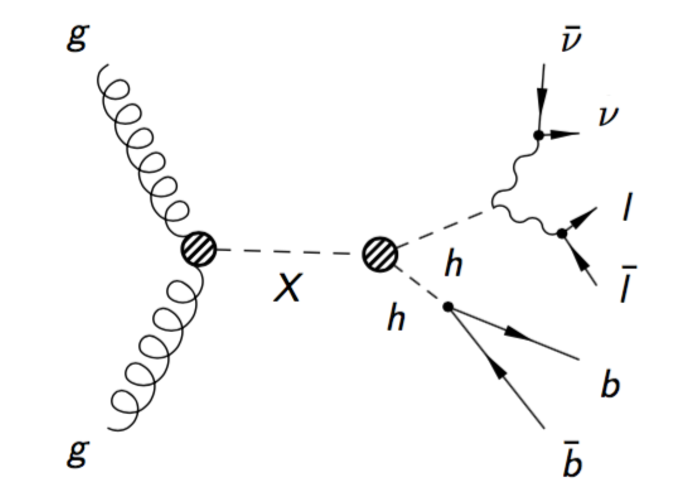
\includegraphics[width=0.45\textwidth]{figures/BGtoHH.pdf}
    \caption{ The Feynman diagram of the graviton production with the subsequent decay to a pair of the Higgs bosons. What follows is a decay to a pair of b quarks and Z bosons. Shown is 2 b quarks, 2 leptons, and 2 neutrinos final state.
    }
    \label{fig:BGtoHH}
  \end{center}
\end{figure}


\subsection{Analysis Strategy}

The analysis is based on ntuples and object selection from the approved VHbb sister analysis~\cite{VHbb_inspire}. Leptons, b jets, and the missing transverse energy (MET) are reconstructed using the standard CMS procedures~\cite{CMSreco} and the Particle Flow (PF) algorithm~\cite{PFalgo}. b-jets are identified using the Combined MVA v2 (CMVA) algorithm~\cite{BTagtwiki}. Then, on shell Z bosons are selected of dilepton pairs with a net charge zero for a pair. Higgs boson decaying to b quarks (Hbb) is reconstructed as a pair of b jets with the highest CMVA output value. Finally, double Higgs boson transverse mass, which is used in the shape analysis to extract limits, is constructed computing the transverse mass of the sum of the Lorentz vectors of the two leptons forming the on-shell Z, MET, and a pair of the b jets forming the \HBB. An additional cut on the missing transverse energy preserves the orthogonality with the existing HIG-18-013 ``2b 2l 2q'' analysis. Lastly, the cut on the BDT is used to reduce the background contamination in the signal region.

Main backgrounds are \ttbar and Drell-Yan in association with jets. Their normalization is extracted during the simultaneous fit of signal region (SR), as well as control region \ttbar (CRTT), and control region Drell-Yan (CRDY). Others, minor backgrounds, are single top production, diboson samples (WW, WZ, ZZ), and ZH production. 
%We assign systematics uncertainties on the QCD scale corresponding to each process. Also uncertainty associated with the imperfect knowledge of the single top cross section is added.
